\documentclass[compress]{beamer}

\usetheme{Hamburg}

\usepackage[utf8]{inputenc}
%\usepackage{units}

\title{NeuGenGo \\ Kann ein neuronales Netz besser Go spielen als wir?}
\author{Lennart Braun, Armin Schaare, Theresa Eimer}
\institute{Praktikum Parallele Programmierung \\Fachbereich Informatik\\Universität Hamburg}
\date{03.06.2015}

\begin{document}

\begin{frame}
	\titlepage
\end{frame}

\begin{frame}
	\frametitle{Gliederung (Agenda)}

	\tableofcontents
\end{frame}

\section{Ziele}

\begin{frame}
	\frametitle{Ziele}
	
	\begin{itemize}
		\item Ein gut spielendes Netz als Ergebnis
		\item Spiele und Netze visualisierbar machen
		\item Einen guten Vererbungsmechanismus finden
	\end{itemize}
	
\end{frame}

\section{Go}

\begin{frame}
	\frametitle{Go - Das Spiel}

	\begin{itemize}
		\item Asiatisches Brettspiel
		\item Wird auf Brettern mit 19x19 Knoten gespielt
		\item Ziel: gleichzeitig Gebiet einkreisen und gegnerische Steine schlagen
		\item Spielende: wenn beide Spieler passen
	\end{itemize}

	\begin{figure}
		\begin{center}
			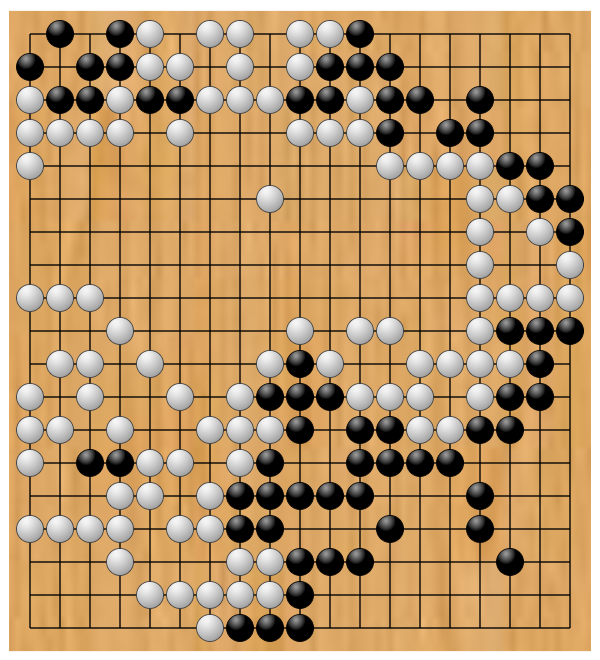
\includegraphics[scale=0.15]{board.png}
		\end{center}
		\caption{Beispiel eines Bretts}
		\begin{footnotesize}		 
		Quelle: http://www.13thmonkey.org/Artdraw/images/kifu2.png
		\end{footnotesize}
		\label{fig:Brett}
	\end{figure}
\end{frame}

\begin{frame}
	\frametitle{Go - Die Umsetzung}
	
	\begin{itemize}
		\item Gespielt wird auf kleineren Brettern (bis 9x9)
		\item Repräsentation als Datentyp mit dem Brett als Array, einem Array zum Speichern von Gruppen und dem als nächstes ziehenden Spieler
		\item Das Spiel endet, wenn es keine gültigen Züge mehr gibt
		\item Das Spielbrett prüft Züge und verhindert Regelverstöße
		\item Ungültige Spielzüge werden auf den nächstbesten erlaubten Zug gesetzt
	\end{itemize}		
	
\end{frame}

\section{Das Netz}

\begin{frame}[fragile]
	\frametitle{Das Netz}

	\begin{itemize}
		\item Neuronales Netz mit...

		\begin{itemize}
			\item ...n+1 Input-Neuronen für n Knoten auf dem Spielfeld, plus der Differenz schwarzer und weißer Steine
			\item ...beliebig vielen hidden layers, die jeweils wieder m Neuronen besitzen
			\item ...2 Output-Neuronen für die x- bzw. y-Koordinate des nächsten Zuges
		\end{itemize}

		\item Ein Neuron gibt sein Signal weiter, wenn das aufsummierte Signal der Neuronen aus der Schicht davor einen festgelegten Wert übersteigt
	\end{itemize}
\end{frame}

\begin{frame}
	\frametitle{Was das Netz kann}
	
	\begin{itemize}
		\item Die Eingangssignale für die nächste Schicht an Neuronen berechnen
		\item Die Signale zu einer gültigen Ausgabe auswerten
		\item Den Aufbau des Netzes ausgeben
	\end{itemize}
	
	\begin{figure}
		\begin{center}
			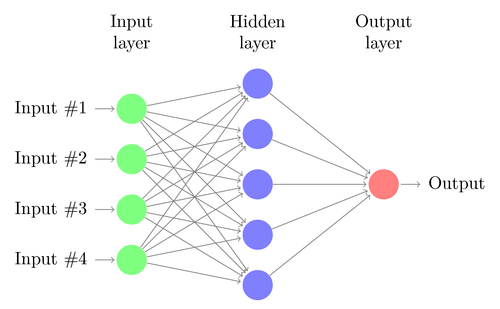
\includegraphics[scale=0.25]{net.png}
		\end{center}
		\caption{Beispielnetz}
		\begin{footnotesize}
		Quelle: http://www.texample.net/media/tikz/examples/PNG/neural-network.png
		\end{footnotesize}
		\label{fig:Netz}
	\end{figure}
	
\end{frame}

\section{Der genetische Algorithmus}
\begin{frame}
	\frametitle{Der genetische Algorithmus}

	\begin{itemize}
		\item Je mehr Spiele ein Netz gewinnt, desto wahrscheinlicher überleben dessen Eigenschaften
		\item Verschiedene Möglichkeiten die Vererbung zu gestalten:

		\begin{itemize}
			\item Variable Lebensdauer von Netzen
			\item Verschiedene Mutationswahrscheinlichkeiten
			\item Crossovers
		\end{itemize}
		
		\item Finden der besten Kombination durch Ausprobieren
	\end{itemize}
\end{frame}

%\section{Zeitplan}

\end{document}
